\documentclass[11pt,letterpaper]{article}

% ---------- packages ----------
\usepackage{iftex}
\ifXeTeX
  \usepackage{fontspec}          % Latin Modern by default
\else
  \usepackage[T1]{fontenc}
  \usepackage[utf8]{inputenc}
  \usepackage{lmodern}
\fi
\usepackage[margin=1in]{geometry}
\usepackage{graphicx}
\usepackage{booktabs,tabularx,longtable,array}
\usepackage{enumitem}
\usepackage[font=small,labelfont=bf]{caption}
\usepackage{float}
\usepackage{amssymb}
\usepackage{textcomp}
\usepackage[hidelinks]{hyperref}
\usepackage{microtype}

\setlist{itemsep=2pt,topsep=3pt}
\setlength{\parindent}{0pt}
\setlength{\parskip}{4pt}
\renewcommand{\arraystretch}{1.2}

\newcommand{\code}[1]{\texttt{\detokenize{#1}}}
\newcommand{\nat}{\textbf{National dataset:}~}
\newcommand{\loc}{\textbf{Local dataset:}~}
\newcommand{\q}[1]{\item \textbf{#1}\par}
\newcolumntype{L}[1]{>{\raggedright\arraybackslash}p{#1}}
\newcolumntype{Y}{>{\raggedright\arraybackslash}X}

\title{Fair Visibility for Local News on Google News Canada\\[4pt]
\large INSE 6450: AI in Systems Engineering, Milestone 1}
\author{
Maria Camila Guzman \\ \small 40239038 \and
David Esuga-Mopah \\ \small 40368321 \and
Ege Karadibak \\ \small 40080456 \and
J. David Ruiz \\ \small 40176885}
\date{Concordia University, Fall 2026 \\ October 19, 2026}

\begin{document}
\maketitle


% =====================================================================
\section{Problem Statement}

\subsection*{Task definition}
Small and independent news outlets can report a story first but still appear below larger publishers covering the same event on Google News. This makes it harder for readers to find the original reporting and for local outlets to reach their audience. Our project looks at how articles about the same story can be ranked to give smaller outlets a fair chance of being seen, while keeping the result relevant and giving credit to the original source when it can be verified.

\begin{itemize}
\q{What is the input to your system?}
The system takes the articles grouped under the same story on Google News Canada's English and French front pages. For each article, the data includes its headline, link, publication time, publisher and position within the story group. It also includes the number of articles in the group, the news section and the time the page was captured. Publisher information, such as ownership and the payment-based groups that separate major outlets from smaller ones, is used to check and adjust visibility. Publication times identify the earliest article in each group, but on their own they cannot confirm which outlet broke the story.

\q{What is the output (prediction/decision/recommendation)?}
A reordered list of the articles covering the same story. The ranking gives smaller outlets fair visibility while keeping the articles relevant and timely. When the original source can be verified, it is clearly credited. The system will be delivered as a Chrome extension.

\q{Is this classification, regression, ranking, retrieval, forecasting, anomaly detection, etc.?}
Ranking: specifically, reranking the articles that cover the same story. The system changes their order to give smaller outlets fair visibility while weighing relevance, timeliness and credit for original reporting.
\end{itemize}

\subsection*{Target user and use case}
\begin{itemize}
\q{Who uses the system and how?}
People who follow Canadian news on Google News, especially readers looking for local coverage. They use the Chrome extension to see articles in an alternative order that gives smaller outlets fair visibility and helps them find the original reporting.

\q{What decision will your system support or automate?}
The order in which articles about the same story are shown to readers. The system weighs relevance and timeliness while giving smaller outlets a fair chance to appear first.
\end{itemize}

\subsection*{Success criteria}
\begin{itemize}
\q{What does ``good performance'' mean in this context?}
The system consistently produces useful rankings that give smaller outlets fair visibility while keeping coverage relevant and timely. It never presents an outlet as the original source when the evidence is unclear. The Chrome extension displays the results without noticeable delay, does not disrupt normal browsing, and handles missing article information without failing.

\q{Name at least 1--2 evaluation metrics you expect to use (even preliminary).}
\begin{itemize}
\item \textbf{Lead ratio for smaller outlets:} how often smaller outlets appear first, divided by how often they would under an equal-chance ranking (1.0 = fair).
\item \textbf{Ranking relevance:} whether relevant articles appear near the top of the reordered results (e.g.\ NDCG@K).
\item \textbf{Response time:} how long the system takes to process the articles and display the reordered results (p50 and p90 latency).
\end{itemize}
\end{itemize}

\subsection*{Final statement (257 words)}
Small and independent news outlets often report a story first, yet on Google News they tend to appear below larger publishers covering the same event. This makes original local reporting harder for readers to find and makes it harder for local outlets to reach their audience. Our system reranks the articles that Google News groups under one story so that smaller outlets get a fair chance of being seen, while keeping results relevant and timely and crediting the original source only when it can be verified.

The input is a story card from Google News Canada's English or French front page: each article's headline, link, publication time, publisher and position, plus the card size, section and capture time. Publisher ownership and payment group (major outlets versus smaller ones, based on Canadian Journalism Collective payments) are used only to audit and adjust visibility, never as scoring features. The output is a reordered list of the card's articles, shown through a Chrome extension. This is a ranking task: reranking within a story.

The target users are Canadians who follow the news on Google News, especially readers looking for local coverage. The system decides the order in which articles about one story are shown to them.

Good performance means rankings that stay relevant and timely, bring smaller outlets' share of lead positions close to an equal-chance baseline, never present an outlet as the original source when the evidence is unclear, and display without noticeable delay. We will measure the lead ratio for smaller outlets, ranking relevance (NDCG@K) and response time.

\subsection*{Implications for data selection}
\begin{itemize}
\q{Which constraints most strongly shaped your dataset choice and why?}
We needed each article's position on the page, because headlines alone cannot show how high an outlet appeared. Historical data in English and French was necessary to compare time periods and language editions. Cost and archive gaps limited what we could collect. We also needed evidence that local stories existed before treating their absence from Google News as a visibility gap.

\q{Which constraints shaped your sampling/splitting plan?}
Download time and archive availability limited historical sampling, so we drew one random snapshot per language edition per two-day period. Local pages cannot be collected for past dates, and a full collection takes several hours, so repeat readings focus on a 40-town sample. Changes over time also led us to compare results across policy periods and to split training and test data by time.

\q{Which constraints shaped your feature engineering approach?}
The available data limits features to headlines, timestamps, story context and publisher information. Since headlines are in English and French, the plan uses multilingual text embeddings. Publication times identify the earliest observed article, but cannot prove who broke the story. Publisher identity and ownership stay out of the article score and are used only for fairness checks and constraints. Historical exposure features must use only past information to avoid leaking future data.
\end{itemize}

% =====================================================================
\section{Data Selection}

\subsection{Datasets}

Table~\ref{tab:datasets} summarizes the four datasets: how each was obtained, its license, its contents and why it fits the problem.

\begin{itemize}
\q{What alternatives did you consider and why didn't you choose them?}
Google has no official Google News API. Scraping and search API services such as SerpApi cost money and return only current results, not results from years back. Only the Internet Archive holds 2022--2026 pages spanning the Meta news block, the Google agreement and the first payments.

\q{Own data collection: collection method and required tools/APIs}
\nat Snapshots are listed with the Internet Archive CDX API and downloaded unmodified (\code{id_} URLs) with Python \code{requests}, one request every 5--8~s, retrying when the Archive answers 503 (\code{collection/01_front_page.ipynb}). Each page embeds its stories as JSON (\code{AF_initDataCallback}, key \code{gbres}), which we parse into one row per article: section, card, slot, headline, outlet and publication time. Outlets are matched to the CJC payment lists and Google's 2024 open-call list with fuzzy name matching (\code{rapidfuzz}); 262 of 654 outlets were checked by hand. For the search check, \code{collection/03_search_links.ipynb} builds the Google News and Google Search links for the 31 stories, and the top 10 results were recorded by hand.

\loc Each town's page is read logged out (so account personalization does not affect the results) with Python \code{requests} in \code{collection/02_local_pages.ipynb}, 30~s apart. Each story card is parsed into rank, headline, outlet, time and link. Stories naming each town come from GDELT bulk files and local outlets' RSS feeds and sitemaps, matched to towns by name.

\q{Own data collection: expected number of samples and feasibility within the course time-frame}
\nat The front-page training data contains 1,474 downloaded snapshots, which take about 2--3 hours to download at 5--8~s each. Collection is complete.

\loc A full pass of 780 Local pages took about 7 hours (Oct 10--11). A Local page can only be read on the current day, since Google keeps no history, so every day without a reading is lost; readings are missing for Oct 14--16.
\end{itemize}

{\small
\begin{longtable}{L{0.12\textwidth} L{0.23\textwidth} L{0.16\textwidth} L{0.21\textwidth} L{0.15\textwidth}}
\caption{Datasets used, how they were obtained and why.}\label{tab:datasets}\\
\toprule
\bfseries Dataset & \bfseries How obtained & \bfseries License / terms & \bfseries Contents & \bfseries Why appropriate \\
\midrule
\endfirsthead
\toprule
\bfseries Dataset & \bfseries How obtained & \bfseries License / terms & \bfseries Contents & \bfseries Why appropriate \\
\midrule
\endhead
\bottomrule
\endfoot
\textbf{Google News front page, 2022--2026} &
The Internet Archive's CDX API lists saved copies of Google News Canada in English and French: about 155,000 English and 64,000 French snapshots from May 2022 to Oct 2026. We drew one random snapshot per edition per 2-day window with a fixed seed (6450): 1,480 drawn, 1,474 downloaded. The JSON embedded in each page is parsed into one row per article. &
\href{https://archive.org/about/terms.php}{Internet Archive Terms of Use} for the CDX API. Articles remain the publishers' property. The downloaded pages stay on our own machines (\code{cache/}) and are not distributed. &
1,336 snapshots in the analysis sample; 16,378 article rows. Fields: \code{timestamp}, \code{edition}, \code{section}, \code{card}, \code{slot} (0 = lead article), \code{cluster_size}, \code{story_id}, \code{outlet}, \code{published_unix}, \code{group}. &
Records where articles were placed before and after the Online News Act. It is the training data for the ranker and the baseline for fair exposure. \\
\midrule
\textbf{Search check, Oct 12, 2026} &
31 stories covered by both a smaller paid outlet and a major one. Each was searched in Google News and in Google Search's News tab using the words both headlines share (no quotes), limited to the story's dates. The top 10 results were recorded. &
Articles remain the publishers' property. &
487 results. Fields: \code{story_id}, \code{engine} (\code{gnews} or \code{gsearch}), \code{rank}, \code{on_story}, \code{size_group}. &
Tests whether Google's search surfaces also put major outlets' stories on top. \\
\midrule
\textbf{Google News Local pages} &
Each town's Local page address encodes its Google Knowledge Graph ID. Pages for 390 towns were read from Google News using these IDs, in English and French: 780 pages on Oct 10--11. &
Articles remain the publishers' property. We store only the card details (headline, source, time, link). &
21,461 story cards (full pass) and 5,481 (repeat readings). A per-town table (394 towns) with cards shown, election stories shown and the outcome. Fields: \code{rank} (position on the page), \code{headline}, \code{source}, \code{time}, \code{link}, \code{town_card}, \code{race_card}, \code{other_town_race}. &
Shows whether a town's own stories appear on its Local page or stay hidden. \\
\midrule
\textbf{Ontario towns} &
2022 municipal results (turnout, acclamations) from the Ministry's official file; 2026 acclamations from AMO. Population and French mother tongue from the 2021 Census. Stories naming each town come from GDELT (Oct 1--9) and about 160 local outlets' RSS feeds and sitemaps (Aug 21 -- Oct 9). The list of local outlets was built from OCNA, Village Media, Postmedia, Réseau.Presse, the CJC list, the Local News Map and Wikipedia. &
GDELT: free to use with citation. Ontario: Open Government Licence. Statistics Canada Open Licence. Outlet feeds are public. &
\code{towns} (414): population, French share, region, coordinates. \code{races_2026} (414): 103 acclaimed mayors. \code{local_outlets}: 1,039 outlets with home town, owner, website. \code{local_stories}: 58,747 story--town matches, with whether the story is about the town's race. \code{civic_outcomes}: 2022 turnout, acclamations, whether the town has its own outlet. &
Tells us which local stories exist, so a story missing from a Local page means ``not shown'', not ``never written''. Also lets us compare towns with and without their own outlet. \\
\end{longtable}
}

\subsection{Data scope and assumptions}
\begin{itemize}
\q{Key assumptions about availability, stationarity, or labeling quality}
\textbf{Availability:} the downloaded snapshots show what logged-out Canadian readers saw at a point in time. Logged-out pages keep account personalization out of the data.

\textbf{Stationarity:} Google's news ranker changes over time. We split the data into policy periods around the Online News Act (before the Meta news block, during the block, after the Google agreement, after CJC payments began) and evaluate each period separately. Local pages change daily and cannot be read for past dates, so each reading is a snapshot of one day; this is why we repeat readings of the 40-town sample.

\textbf{Labeling quality:} all election cards were checked by hand. Stories are matched to towns by name, which can mismatch towns with common names.

\q{Known dataset limitations (coverage gaps, biases, proxies, outdatedness, etc.)}
\begin{itemize}
\item The front-page dataset has no snapshots in either edition from June to September 2022, and no French snapshots in September 2023 and June 2026 (Figure~\ref{fig:snapshots}).
\item Position on the page is a proxy for exposure: it shows what was displayed, not what was read. There is no click data.
\item Outlet groups use Year 2 CJC payments for the whole 2022--2026 period.
\item The search check covers 31 stories, recorded from one signed-in account in Montreal.
\item Local data covers Ontario only, one election and a few days of readings.
\item GDELT misses some outlets, so outlet feeds were added.
\end{itemize}
\end{itemize}

\subsection{Data report}

\subsubsection{Missingness summary}
\nat
\begin{itemize}
\item Of the 1,480 drawn snapshots, 6 could not be downloaded and 5 more were excluded because the Archive served a page more than 3 hours from the requested time.
\item There are no snapshots in either edition from June to September 2022, and no French snapshots in September 2023 and June 2026 (Figure~\ref{fig:snapshots}).
\item \code{story_id} is empty for 47.2\% of article rows. This is structural: single-article cards have no story ID. It is more frequent in older pages (59.4\% in 2022 vs.\ 42.6\% in 2026).
\item \code{cjc_sub} and \code{payee_legal} are empty for 20.9\% of articles, because those outlets received no CJC payment. 64.4\% of the 654 outlets in \code{outlets.csv} have no CJC payee match, and 157 outlets are in the group \code{unknown}.
\item In the search check, the publication time is empty for 51\% of results (Google Search shows no exact time), and the major outlet's time is missing for 12 of the 31 stories.
\end{itemize}

\loc
\begin{itemize}
\item 4 of the 394 towns were not collected, so their card counts are empty.
\item No French cards were captured for 256 of the 390 towns that were read.
\item 4 columns of \code{local_page_by_town} are empty for every town.
\item \code{other_town_race} is empty for 96\% of cards by design: it is only filled when a card is about another town's election.
\item 2022 turnout is missing for 32 towns, all with a fully acclaimed council.
\item 41\% of local outlets have no website (mostly print and radio), and 1\% of stories have no title.
\end{itemize}

\subsubsection{Summary statistics for important fields}
\nat
\begin{itemize}
\item 16,378 article rows from the 1,336 snapshots in the analysis sample.
\item The top 10 of the 611 outlets in the sample hold 59.1\% of all slots: La Presse 1,427, Journal de Montréal 1,387, CBC 1,358.
\item Lead articles by outlet group: major 78.6\%, foreign 14.9\%, local English 2.2\%, Canadian unpaid 1.7\%, francophone 1.6\%, unknown 0.9\% (Figure~\ref{fig:groups}).
\item 487 results were collected in the search check; 84.6\% are about the story that was searched.
\end{itemize}

\loc Towns where an election story about them exists, by population: 30 under 2,000; 81 at 2,000--9,999; 92 at 10,000--49,999; 42 at 50,000+. The share of these towns whose election story appears on their Local page is 23\%, 52\%, 78\% and 93\% respectively (Figure~\ref{fig:local}). Among towns under 10,000, the mayor was acclaimed in 77 of 224 towns without their own outlet (34\%), vs.\ 6 of 39 towns with one (15\%) (Figure~\ref{fig:acclaimed}).

\subsubsection{Duplicates and outliers}
\nat No link appears twice in the same snapshot. The 133 same-day repeat snapshots are flagged in \code{snapshots.csv} (\code{purpose = repeat}) and kept out of the analysis sample. We compared two times for each article: the capture time (when the Internet Archive saved the page) and the publication time (when Google says the article was published). 7 articles were published after the capture time and 33 were more than 7 days old.

\loc Some stories match several towns, and syndicated copies repeat the same title. We count each story once per town.

\subsubsection{Example rows}

\begin{table}[H]
\centering\footnotesize
\resizebox{\textwidth}{!}{%
\begin{tabular}{@{}l l L{2.1cm} c c c L{5.6cm} l l r@{}}
\toprule
\bfseries timestamp & \bfseries edition & \bfseries section & \bfseries card & \bfseries slot & \bfseries size & \bfseries headline & \bfseries outlet & \bfseries group & \bfseries cjc\_y2 (\$) \\
\midrule
20260117022450 & en-CA & Top stories & 1 & 0 & 4 & Blair and Rubio among names on Gaza `Board of \ldots & bbc.com & foreign & 0 \\
20260117022450 & en-CA & Top stories & 1 & 1 & 4 & Carney to accept Trump's offer for role on Gaz\ldots & ctvnews.ca & major & 8,646,776 \\
20260117022450 & en-CA & Top stories & 1 & 2 & 4 & CP NewsAlert: Carney to join Trump's `Board of\ldots & panow.com & local\_en & 584,854 \\
20260522004240 & fr-CA & À la une & 0 & 0 & 4 & Des Canadiens iront aider la République démocr\ldots & granbyexpress.com & franco & 931,762 \\
20260522004240 & fr-CA & Sélections pour vous & 0 & 0 & 1 & Il aurait drogué une femme dans un bar pour l'\ldots & journaldemontreal.com & major & 2,398,348 \\
\bottomrule
\end{tabular}}
\caption{Example rows from the national dataset (\code{front_page_articles.csv}).}
\end{table}

\begin{table}[H]
\centering\footnotesize
\resizebox{\textwidth}{!}{%
\begin{tabular}{@{}l l c L{5.8cm} l l c c@{}}
\toprule
\bfseries town\_id & \bfseries edition & \bfseries rank & \bfseries headline & \bfseries source & \bfseries time & \bfseries race\_card & \bfseries other\_town\_race \\
\midrule
3502044 & fr-CA & 16 & Un conseiller de Casselman veut faire le saut \ldots & Le Droit & 2026-01-18T08:00:00Z & True & (empty) \\
3511005 & en-CA & 59 & Six questions with Paul Proderick, candidate f\ldots & Kingstonist News & 2026-09-24T07:00:00Z & True & (empty) \\
3501005 & en-CA & 2 & Homelessness the top issue at Cornwall mayoral\ldots & Cornwall Standard Freeholder & 2026-10-09T20:44:03Z & False & 3501012 \\
\bottomrule
\end{tabular}}
\caption{Example rows from the local dataset (\code{local_page_cards.csv}).}
\end{table}

\subsubsection{Plots}

\begin{figure}[H]
\centering
\begin{minipage}[t]{0.55\textwidth}\centering
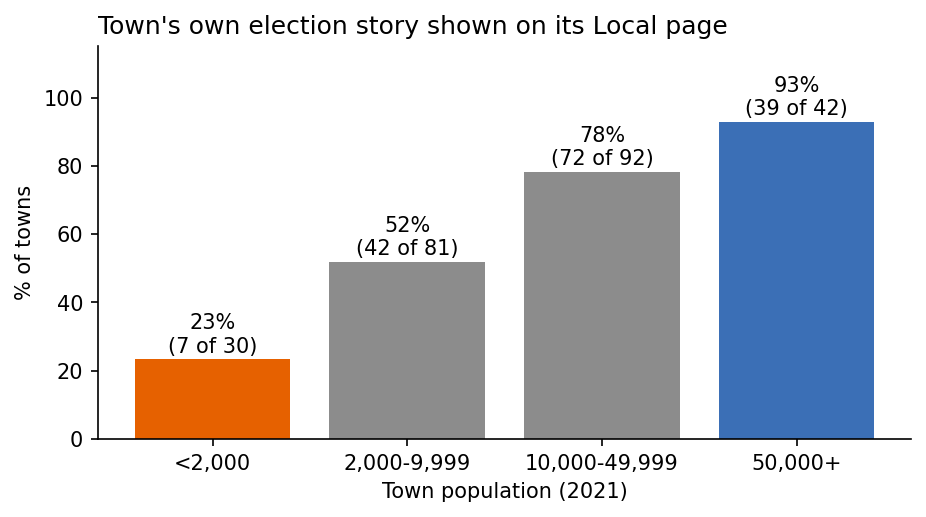
\includegraphics[width=\linewidth]{figures/fig1_local_pages_by_town_size.png}
\caption{Town's own election story shown on its Local page, by town population.}\label{fig:local}
\end{minipage}\hfill
\begin{minipage}[t]{0.40\textwidth}\centering
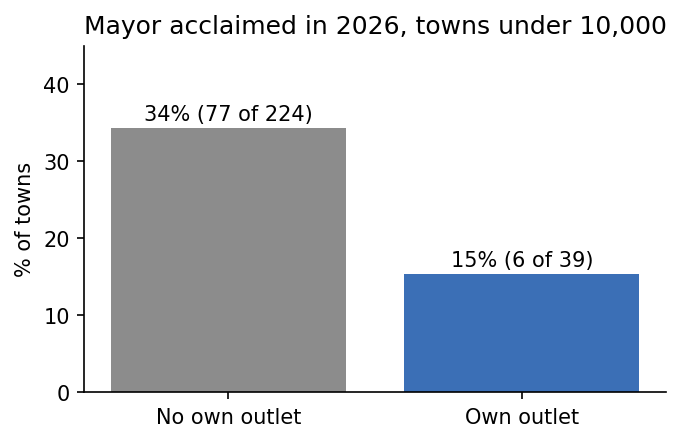
\includegraphics[width=\linewidth]{figures/fig2_acclaimed_mayors.png}
\caption{Mayor acclaimed in 2026, towns under 10,000 people.}\label{fig:acclaimed}
\end{minipage}
\end{figure}

\begin{figure}[H]
\centering
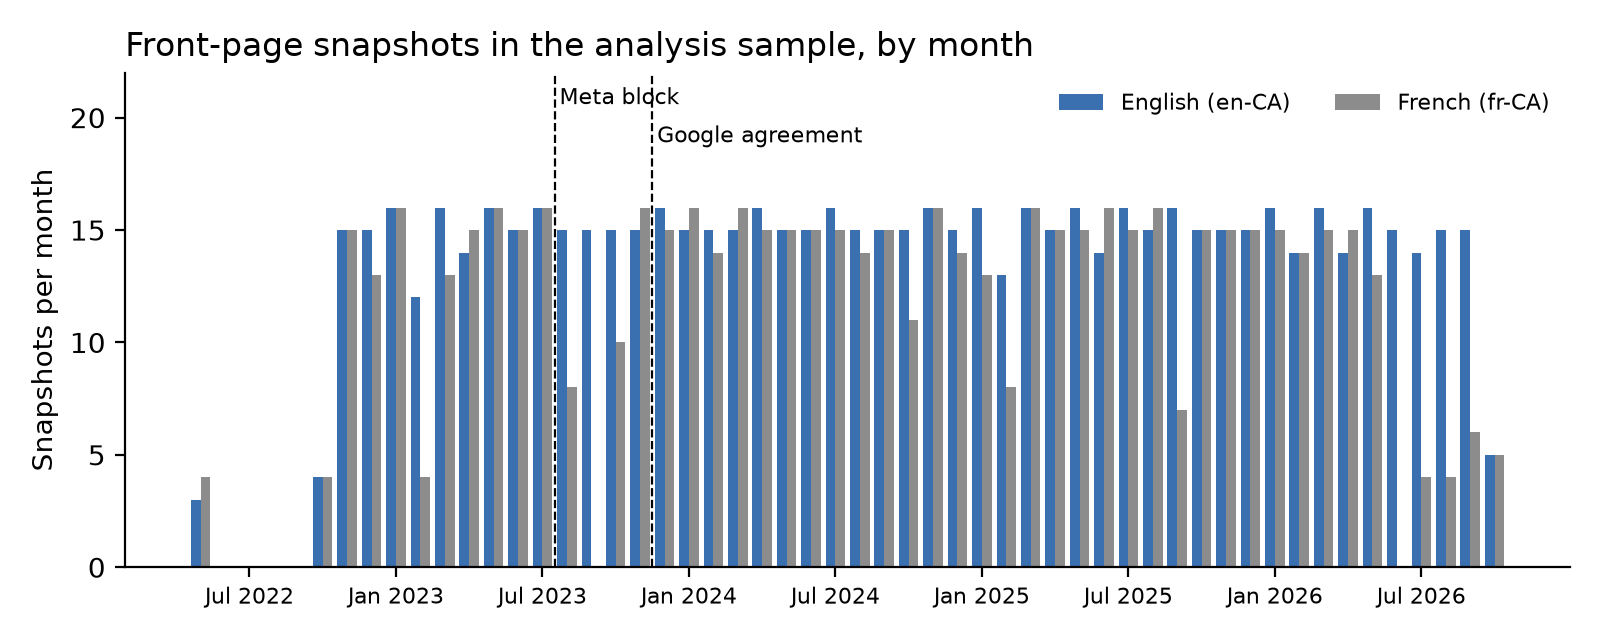
\includegraphics[width=0.92\textwidth]{figures/fig3_snapshots_per_month.png}
\caption{Front-page snapshots in the analysis sample, per month and edition.}\label{fig:snapshots}
\end{figure}

\begin{figure}[H]
\centering
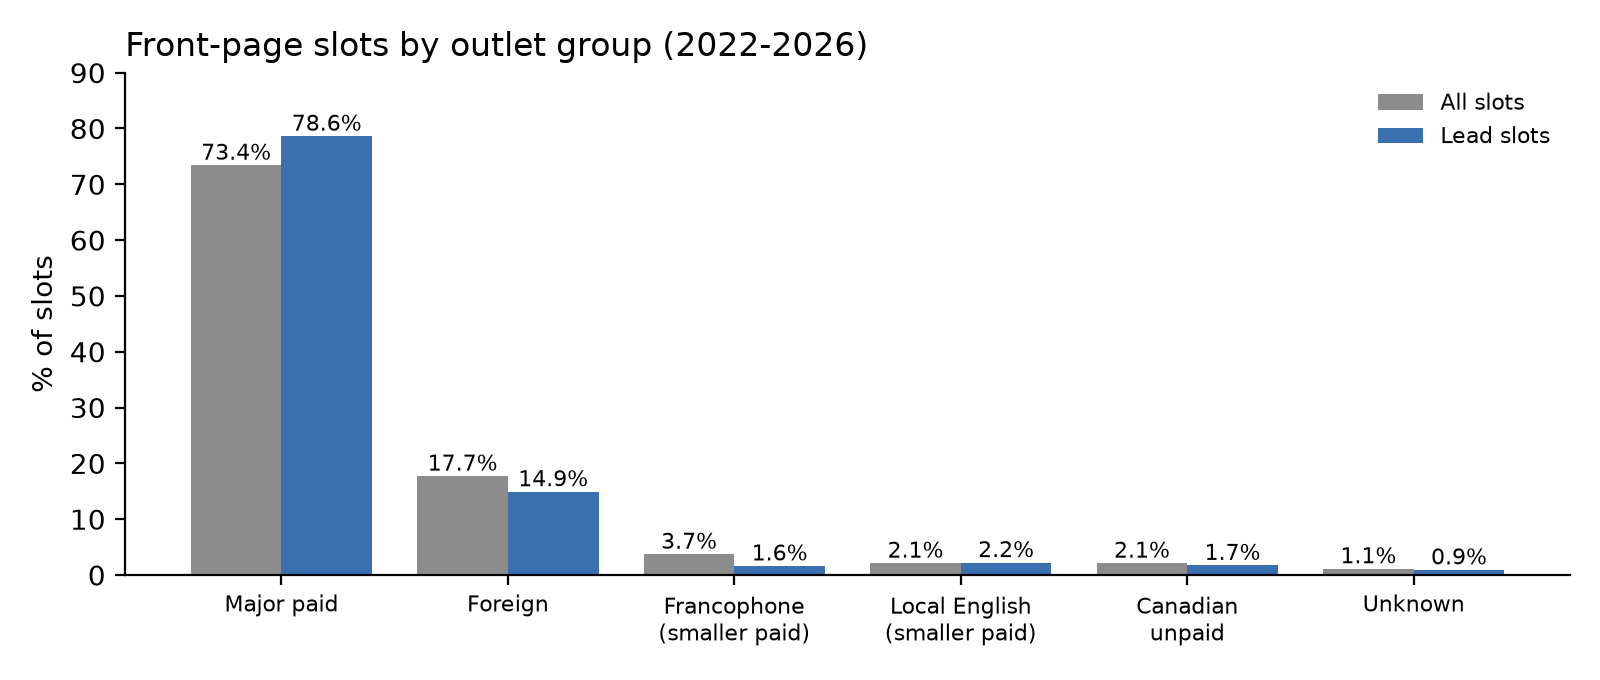
\includegraphics[width=0.92\textwidth]{figures/fig4_slots_by_group.png}
\caption{Share of all front-page slots and of lead slots, by outlet group.}\label{fig:groups}
\end{figure}

\clearpage
\subsection{Data issues and handling plan}

{\small
\begin{longtable}{L{0.16\textwidth} L{0.38\textwidth} L{0.37\textwidth}}
\caption{Data issues and how we handle them.}\label{tab:issues}\\
\toprule
\bfseries Issue & \bfseries Present in our data? (where) & \bfseries Plan to handle it (or why it doesn't apply) \\
\midrule
\endfirsthead
\toprule
\bfseries Issue & \bfseries Present in our data? (where) & \bfseries Plan to handle it (or why it doesn't apply) \\
\midrule
\endhead
\bottomrule
\endfoot
\textbf{Missing values} &
\nat 11 snapshots not downloaded or excluded. Month-long gaps in 2022, and in the French edition in 2023 and 2026. \code{story_id} is empty for 47.2\% of article rows. Unpaid outlets have no CJC match.

\loc Empty columns, 4 towns not collected, no French cards for most towns (256 of 390), no turnout where the council was acclaimed. &
\nat Use only the main downloaded snapshots. Identify story groups by snapshot, card and slot instead of \code{story_id}. Treat ``no CJC match'' as unpaid, not as missing.

\loc Drop the empty columns and the 4 towns. Analyse English and French separately. Leave turnout empty, with an ``acclaimed'' flag. \\
\midrule
\textbf{Inconsistent formats / units} &
\nat Archive timestamps as \code{YYYYMMDDhhmmss}, publication times as Unix seconds. One company can be registered under several names or websites (e.g.\ Québecor appears under 3 legal names: MédiaQMI inc., Groupe TVA inc., NumériQ inc.).

\loc Card times in ISO format, story dates as \code{YYYYMMDDhhmmss}; one outlet under two names (e.g.\ ``The Kincardine Record'' / kincardinerecord.ca). &
\textbf{National and local datasets:} Convert all times to UTC. Map outlet names to their website, and group legal names under their parent company. \\
\midrule
\textbf{Label noise or weak labels} &
\nat Outlet groups come from fuzzy name matching. Off-story search results were labelled by hand. The earliest publication time does not prove who broke a story.

\loc Towns are matched by name, and some town names are ambiguous. &
\nat Keep the 262 hand-checked outlet tags and report \code{unknown} outlets (0.9\% of slots) as their own group. Drop off-story search results. Call the earliest article the ``first observed'' one, not the original source, and credit an original source only when it is verified by hand.

\loc Keep the hand-checked election tags, compare strict and loose election tags, and rerun without ambiguous towns. \\
\midrule
\textbf{Outliers and erroneous values} &
\nat 5 snapshots served from another date (up to 124 hours off). 7 articles published after the capture time (by at most 1.4 hours) and 33 articles more than 7 days old.

\loc Very old cards; Toronto has 18,397 stories. &
\nat Drop the 5 snapshots (more than 3 hours off). Set the 7 small negative ages to zero (clock differences). Flag ages over 7 days as wrong timestamps and leave them out of timing features.

\loc Keep card age as a variable; use a log scale for population and story counts. \\
\midrule
\textbf{Duplicate values} &
\nat 133 same-day repeat snapshots.

\loc Repeated links, syndicated stories. &
\nat Keep the repeat snapshots only as a stability check. Count each link once per page.

\loc Count each link once per page and each title once per town. \\
\midrule
\textbf{Data drift risk} &
\nat Google's ranker and the policy setting change over 2022--2026 (Meta news block, Google agreement, CJC payments).

\loc Pages change daily, and missed days cannot be recovered. &
\nat Split training and test sets by time and policy period, not at random.

\loc Daily readings until Nov 2; report results per day. \\
\midrule
\textbf{Class imbalance} &
\nat Major outlets hold 78.6\% of lead slots; smaller outlets have under 4\% of leads.

\loc Election cards are rare (360 of 21,461), and 239 of the 390 towns have under 10,000 people. &
\nat Report results per outlet group with exact counts and compare them to the equal-chance baseline.

\loc Report results by town-size group with exact counts. \\
\midrule
\textbf{Labelling (if unsupervised)} &
\nat Does not apply: the task is supervised. The lead slot on Google's page is the label, and the other labels are the hand-checked outlet groups and on-story tags.

\loc Does not apply: no model is trained on it. Local results are comparisons of stories shown vs.\ stories that exist. &
Not applicable. \\
\end{longtable}
}

% =====================================================================
\section{Feature Engineering}

\subsection*{Candidate features}
{\small
\begin{tabularx}{\textwidth}{@{}L{0.14\textwidth} L{0.25\textwidth} Y L{0.22\textwidth}@{}}
\toprule
\bfseries Family & \bfseries Source & \bfseries Feature & \bfseries Role \\
\midrule
Timing & \code{front_page_articles.csv} & time since first publication in the cluster; is-first-published flag & Merit: fed to the score \\
Headline content & \code{front_page_articles.csv} & multilingual headline embedding; headline length & Merit: fed to the score \\
Story context & \code{front_page_articles.csv} & cluster size, section, edition, card position & Merit: fed to the score \\
Outlet identity and resourcing & \code{outlets.csv} & group (major / local / foreign), CJC payment amount, outlet's slot frequency, owner / parent company & Constraint only: audits and calibrates the score, never a model input \\
Ownership graph & \code{outlets.csv} & ownership concentration (HHI) per story cluster; outlet co-occurrence centrality & Constraint only: same as above \\
Policy-era context & derived from \code{timestamp} & days since each Online News Act milestone (Meta block, Google deal, CJC payments) & Evaluation only: tracks the trend, not a score input \\
\bottomrule
\end{tabularx}
}

\subsection*{Feature types}
{\small
\begin{tabularx}{\textwidth}{@{}L{0.2\textwidth} Y L{0.38\textwidth}@{}}
\toprule
\bfseries Type & \bfseries Example & \bfseries Role \\
\midrule
Numeric & time since first publication, cluster size & Merit: fed to the score \\
Text embedding & headline (bilingual) & Merit: fed to the score \\
Categorical & edition, section & Merit: fed to the score \\
Categorical (protected) & outlet group, outlet domain & Constraint only: not fed to the score \\
Graph & ownership concentration (HHI), outlet co-occurrence centrality & Constraint only: not fed to the score \\
Time-window aggregate & trailing lead rate per outlet & Constraint only: audits and calibrates exposure, never a score input \\
\bottomrule
\end{tabularx}
}

\subsection*{Domain-specific transformations}
{\small
\begin{tabularx}{\textwidth}{@{}L{0.2\textwidth} L{0.27\textwidth} Y@{}}
\toprule
\bfseries Transformation & \bfseries Applied to & \bfseries Why \\
\midrule
Log scaling (\code{log1p}) & CJC payment amount, outlet slot count & Heavy right skew: a few major outlets dominate. \\
Policy-relative time & \code{timestamp} \textrightarrow{} days since each Online News Act milestone & The deal's effect is relative to the milestones, not to the calendar date. \\
Causal rolling average & trailing per-outlet lead rate & Used only to audit and calibrate exposure (constraint role), never fed to the score. The window must only look backward, or it leaks the target. \\
\bottomrule
\end{tabularx}
}

\subsection*{Handling of categorical variables}
{\small
\begin{tabularx}{\textwidth}{@{}L{0.2\textwidth} L{0.13\textwidth} Y@{}}
\toprule
\bfseries Variable & \bfseries Cardinality & \bfseries Treatment \\
\midrule
Edition (en / fr) & 2 & Binary, fed to the score. \\
Outlet group & 6 & Fairness-constraint variable only: held out of the score, used to calibrate exposure toward equal chance. \\
Outlet domain & hundreds (611 in the sample) & Fairness-constraint variable only: no target-encoded historical lead rate (that would be circular); the domain only groups outlets for calibration. \\
Owner / parent company & dozens & Folded into the ownership-concentration (HHI) constraint feature, not encoded as a score input. \\
\bottomrule
\end{tabularx}
}

\subsection*{Handling of text, images and audio}
Headlines are short and bilingual (English and French). We will normalize them and embed them with a multilingual sentence-embedding model (LaBSE or a multilingual MiniLM), so that matching French and English headlines land close together in vector space. No images or audio are captured, so both are out of scope.

% =====================================================================
\section{Code Submission}
\begin{itemize}
\item GitHub repository created and shared with the TA and the instructor: \url{https://github.com/GitExcited/Behind-the-Feed-Data-Challenge}
\item \code{README.md}: how to run the code, dependencies, and where outputs are saved
\item Code runs from raw data
\item Code is clear and commented
\item No hard-coded absolute paths
\item Saved output artifacts in \code{outputs/}: the six result charts made by \code{main_findings.ipynb} (PNG) and the missing-value table \code{local_missingness.csv}
\end{itemize}

\end{document}
